\documentclass[aspectratio=169, 10pt]{beamer}

% ─── Packages ───────────────────────────────────────────────────────────────
\usepackage[utf8]{inputenc}
\usepackage[T1]{fontenc}
\usepackage{lmodern}
\usepackage{microtype}
\usepackage{xcolor}
\usepackage{listings}
\usepackage{hyperref}
\usepackage{tikz}
\usetikzlibrary{shapes.geometric, arrows.meta, positioning, fit, shadows.blur, calc}
\usepackage{booktabs}
\usepackage{tabularx}

% ─── Color Palette Definitions ──────────────────────────────────────────────
\definecolor{axonpurple}{RGB}{108, 99, 255}
\definecolor{axondark}{RGB}{24, 24, 37}
\definecolor{axongold}{RGB}{198, 138, 0}
\definecolor{codegreen}{RGB}{40, 160, 40}
\definecolor{codegray}{RGB}{120, 120, 120}
\definecolor{codebg}{RGB}{245, 245, 248}

% ─── Beamer Theme Customization ─────────────────────────────────────────────
\usetheme{Madrid}
\usecolortheme{default}
\useinnertheme{circles}

\setbeamercolor{structure}{fg=axonpurple}
\setbeamercolor{palette primary}{bg=axonpurple, fg=white}
\setbeamercolor{palette secondary}{bg=axonpurple!80!black, fg=white}
\setbeamercolor{palette tertiary}{bg=axonpurple!60!black, fg=white}
\setbeamercolor{palette quaternary}{bg=axondark, fg=white}
\setbeamercolor{titlelike}{parent=palette primary, fg=white}
\setbeamercolor{frametitle}{bg=axonpurple, fg=white}
\setbeamercolor{block title}{bg=axonpurple, fg=white}
\setbeamercolor{block body}{bg=axonpurple!8, fg=black}

\setbeamertemplate{navigation symbols}{} % Hide navigation buttons
\setbeamertemplate{headline}{}

% Custom footer layout
\setbeamertemplate{footline}{
  \leavevmode%
  \hbox{%
  \begin{beamercolorbox}[wd=.333333\paperwidth,ht=2.25ex,dp=1ex,center]{palette quaternary}%
    \usebeamerfont{author in head/foot}Galgotias University
  \end{beamercolorbox}%
  \begin{beamercolorbox}[wd=.333333\paperwidth,ht=2.25ex,dp=1ex,center]{palette secondary}%
    \usebeamerfont{title in head/foot}Axon Flow: Academic Presentation
  \end{beamercolorbox}%
  \begin{beamercolorbox}[wd=.333333\paperwidth,ht=2.25ex,dp=1ex,right]{palette primary}%
    \usebeamerfont{date in head/foot}\insertshortdate{}\hspace*{2em}
    \insertframenumber{} / \inserttotalframenumber\hspace*{2ex}
  \end{beamercolorbox}}%
  \vskip0pt%
}

% ─── Listings (Code Styling) Setup ─────────────────────────────────────────
\lstdefinelanguage{javascript}{
  keywords={typeof, new, true, false, catch, function, return, null, catch, switch, var, if, in, while, do, else, case, break, const, let},
  keywordstyle=\color{axonpurple}\bfseries,
  ndkeywords={class, export, boolean, throw, implements, import, this},
  ndkeywordstyle=\color{axonpurple}\bfseries,
  identifierstyle=\color{black},
  sensitive=false,
  comment=[l]{//},
  morecomment=[s]{/*}{*/},
  commentstyle=\color{codegreen},
  stringstyle=\color{axongold},
  morestring=[b]',
  morestring=[b]"
}

\lstdefinelanguage{json}{
  keywords={true, false, null},
  keywordstyle=\color{axonpurple}\bfseries,
  string=[s]{"}{"},
  stringstyle=\color{axongold},
  comment=[l]{:},
  commentstyle=\color{black}
}

\lstset{
  basicstyle=\ttfamily\scriptsize,
  backgroundcolor=\color{codebg},
  keywordstyle=\color{axonpurple}\bfseries,
  commentstyle=\color{codegreen},
  stringstyle=\color{axongold},
  frame=single, 
  rulecolor=\color{black!10},
  breaklines=true, 
  showstringspaces=false,
  tabsize=2
}

% ─── Presentation Info ──────────────────────────────────────────────────────
\title[\textbf{Axon Flow}]{\Huge \textbf{Axon Flow}}
\subtitle{A Performant Hierarchical Mind-Mapping Platform \\ using Client-Side D3-Layouts and Optimistic UI}
\author[Akshat Raj \& Pavan Soni]{\textbf{Akshat Raj} (23scse1010833) \\ \textbf{Pavan Soni} (23scse1012576)}
\institute[GU]{Department of Computer Science \& Engineering \\ Galgotias University}
\date{\today}

% ════════════════════════════════════════════════════════════════════════════
\begin{document}

% ─── Slide 1: Title Slide ──────────────────────────────────────────────────
\begin{frame}[plain]
  \titlepage
\end{frame}

% ─── Slide 2: What is Axon Flow? ───────────────────────────────────────────
\begin{frame}{Project Overview: What is Axon Flow?}
  \begin{columns}
    \begin{column}{0.55\textwidth}
      \textbf{Axon Flow} is a full-stack, browser-native mind-mapping application designed for seamless brainstorming and knowledge organization.
      \vspace{0.4em}
      \begin{itemize}
        \item[\textcolor{axonpurple}{\tiny$\blacksquare$}] \textbf{Infinite Canvas}: Dynamic panning and zooming to view and manage large concept trees.
        \item[\textcolor{axonpurple}{\tiny$\blacksquare$}] \textbf{Auto-Layout Modes}: Nodes automatically reposition into Horizontal, Vertical, or Radial hierarchies.
        \item[\textcolor{axonpurple}{\tiny$\blacksquare$}] \textbf{Smart Client Architecture}: Relational hierarchy is resolved to physical positions entirely on the user's browser.
      \end{itemize}
    \end{column}
    \begin{column}{0.45\textwidth}
      \begin{block}{Technology Stack}
        \textbf{Frontend}: React 18, React Flow (\texttt{@xyflow/react}), D3-Hierarchy\\
        \textbf{Backend}: Node.js + Express.js (REST API)\\
        \textbf{Database}: MongoDB Atlas (Mongoose ODM)\\
        \textbf{Auth}: Clerk (JWT-based secure isolation)
      \end{block}
    \end{column}
  \end{columns}
\end{frame}

% ─── Slide 3: Visual Concept of Axon Flow ──────────────────────────────────
\begin{frame}{Mind Map Visual Topology}
  \begin{columns}
    \begin{column}{0.5\textwidth}
      \textbf{Core Topology of Axon Flow}:
      \vspace{0.6em}
      \begin{itemize}
        \item[\textcolor{axonpurple}{\tiny$\blacksquare$}] \textbf{Radial and Orthogonal Layouts}: Clean, automated fanning out of nodes from a central root.
        \item[\textcolor{axonpurple}{\tiny$\blacksquare$}] \textbf{Custom Nodes (Leaves)}: Rich nodes holding independent attributes (files, code files, and links).
        \item[\textcolor{axonpurple}{\tiny$\blacksquare$}] \textbf{Re-parenting Paths}: Drag-and-drop actions automatically calculate new connection curves.
      \end{itemize}
    \end{column}
    \begin{column}{0.5\textwidth}
      \begin{center}
        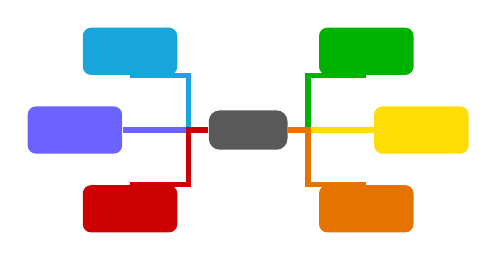
\begin{tikzpicture}[
          root/.style={rectangle, rounded corners=4pt, fill=gray!70!black, minimum width=1.0cm, minimum height=0.5cm, draw=none},
          nodecyan/.style={rectangle, rounded corners=3pt, fill=cyan!90!black, minimum width=1.2cm, minimum height=0.6cm, draw=none},
          nodegreen/.style={rectangle, rounded corners=3pt, fill=green!70!black, minimum width=1.2cm, minimum height=0.6cm, draw=none},
          nodepurple/.style={rectangle, rounded corners=3pt, fill=axonpurple, minimum width=1.2cm, minimum height=0.6cm, draw=none},
          nodeyellow/.style={rectangle, rounded corners=3pt, fill=yellow!80!orange, minimum width=1.2cm, minimum height=0.6cm, draw=none},
          nodered/.style={rectangle, rounded corners=3pt, fill=red!80!black, minimum width=1.2cm, minimum height=0.6cm, draw=none},
          nodeorange/.style={rectangle, rounded corners=3pt, fill=orange!90!black, minimum width=1.2cm, minimum height=0.6cm, draw=none},
          conn/.style={thick, line width=2pt}
        ]
          % Central Root
          \node[root] (root) at (0,0) {};

          % Surrounding Nodes
          \node[nodecyan] (cyan) at (-1.5, 1.0) {};
          \node[nodegreen] (green) at (1.5, 1.0) {};
          
          \node[nodepurple] (purple) at (-2.2, 0) {};
          \node[nodeyellow] (yellow) at (2.2, 0) {};
          
          \node[nodered] (red) at (-1.5, -1.0) {};
          \node[nodeorange] (orange) at (1.5, -1.0) {};

          % Connections
          \draw[conn, cyan!90!black] (root.west) -- ++(-0.25, 0) |- (cyan.south);
          \draw[conn, green!70!black] (root.east) -- ++(0.25, 0) |- (green.south);
          
          \draw[conn, axonpurple] (root.west) -- (purple.east);
          \draw[conn, yellow!80!orange] (root.east) -- (yellow.west);
          
          \draw[conn, red!80!black] (root.west) -- ++(-0.25, 0) |- (red.north);
          \draw[conn, orange!90!black] (root.east) -- ++(0.25, 0) |- (orange.north);
        \end{tikzpicture}
      \end{center}
    \end{column}
  \end{columns}
\end{frame}

% ─── Slide 4: Limitations of Existing Tools ────────────────────────────────
\begin{frame}{Architectural Weaknesses in Standard Tools}
  Most existing web-based mind-mapping platforms suffer from three major design and architectural flaws:
  \vspace{0.5em}
  \begin{enumerate}
    \item \textbf{Nested-Document Storage}:
      \begin{itemize}
        \item Storing the entire tree in a single, deeply nested database document.
        \item \textit{Consequence}: Changing a single node requires writing back the entire heavy tree, leading to high write costs and sync issues.
      \end{itemize}
    \item \textbf{Heavy DOM Re-rendering}:
      \begin{itemize}
        \item Rendering nodes using nested HTML elements (\texttt{div} tags) or raw canvasses that repaint completely when nodes move.
        \item \textit{Consequence}: Severe performance drops, screen flashing, and lag when maps exceed 100 nodes.
      \end{itemize}
    \item \textbf{Lack of Contextual Media Support}:
      \begin{itemize}
        \item Nodes are limited to plain text, lacking ability to bind external files, links, or outlines.
      \end{itemize}
  \end{enumerate}
\end{frame}

% ─── Slide 5: Architectural Disadvantages Visualized ───────────────────────
\begin{frame}{Traditional Database \& DOM Bottlenecks}
  \begin{columns}
    \begin{column}{0.48\textwidth}
      \begin{block}{Nested Document Storage (Database)}
        \centering
        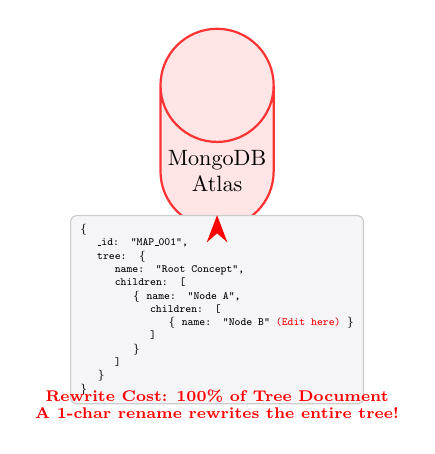
\begin{tikzpicture}[
          scale=0.8, every node/.style={transform shape},
          db/.style={cylinder, shape border rotate=90, draw=red!80, fill=red!10, thick, minimum width=1.6cm, minimum height=1.0cm, align=center},
          jsonbox/.style={rectangle, draw=gray!40, fill=codebg, rounded corners=2pt, font=\ttfamily\tiny, align=left, inner sep=4pt}
        ]
          % Database cylinder
          \node[db] (database) at (0, 1.3) {MongoDB\\Atlas};
          
          % Document structure
          \node[jsonbox] (json) at (0, -0.9) {
            \{ \\
            ~~~\_id: "MAP\_001", \\
            ~~~tree: \{ \\
            ~~~~~~name: "Root Concept", \\
            ~~~~~~children: [ \\
            ~~~~~~~~~\{ name: "Node A", \\
            ~~~~~~~~~~~~children: [ \\
            ~~~~~~~~~~~~~~~\{ name: "Node B" \textcolor{red}{\textbf{(Edit here)}} \} \\
            ~~~~~~~~~~~~] \\
            ~~~~~~~~~\} \\
            ~~~~~~] \\
            ~~~\} \\
            \}
          };
          
          \draw[-Stealth, red, line width=1.5pt] (database) -- (json);
          \node[red, align=center, font=\scriptsize\bfseries] at (0, -2.4) {
            Rewrite Cost: \textbf{100\% of Tree Document} \\
            A 1-char rename rewrites the entire tree!
          };
        \end{tikzpicture}
      \end{block}
    \end{column}
    \begin{column}{0.48\textwidth}
      \begin{block}{Heavy DOM Re-rendering (Browser)}
        \centering
        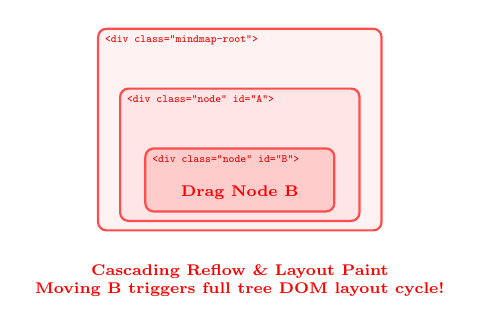
\begin{tikzpicture}[
          scale=0.8, every node/.style={transform shape},
          dombox/.style={rectangle, draw=red!70, fill=red!5, thick, rounded corners=3pt, align=left, inner sep=6pt},
          domlabel/.style={font=\ttfamily\tiny, color=red!90!black}
        ]
          % Root div
          \node[dombox, minimum width=4.5cm, minimum height=3.2cm] (domroot) at (0, 0) {};
          \node[anchor=north west, domlabel] at (domroot.north west) {<div class="mindmap-root">};
          
          % Node A div
          \node[dombox, fill=red!10, minimum width=3.8cm, minimum height=2.1cm] (domnodeA) at (0, -0.4) {};
          \node[anchor=north west, domlabel] at (domnodeA.north west) {<div class="node" id="A">};
          
          % Node B div
          \node[dombox, fill=red!20, minimum width=3.0cm, minimum height=1.0cm] (domnodeB) at (0, -0.8) {};
          \node[anchor=north west, domlabel] at (domnodeB.north west) {<div class="node" id="B">};
          \node[red, font=\scriptsize\bfseries, align=center] at (0, -1.0) {Drag Node B};
          
          \node[red, align=center, font=\scriptsize\bfseries] at (0, -2.4) {
            Cascading Reflow \& Layout Paint \\
            Moving B triggers full tree DOM layout cycle!
          };
        \end{tikzpicture}
      \end{block}
    \end{column}
  \end{columns}
\end{frame}

% ─── Slide 6: How Axon Flow Differs from the Rest ──────────────────
\begin{frame}{Axon Flow Core Architecture}
  \begin{columns}
    \begin{column}{0.5\textwidth}
      \begin{block}{1. Flat-Tree Data Model}
        Every node is stored in MongoDB as an \textbf{independent flat document}. 
        \begin{itemize}
          \item[\checkmark] Scoped to a map via \texttt{mapId}.
          \item[\checkmark] Linked strictly via a \texttt{parentId} reference.
          \item[\checkmark] Updating a node name or collapsing a branch modifies only \textbf{one} database record (\texttt{PATCH}).
        \end{itemize}
      \end{block}
    \end{column}
    \begin{column}{0.5\textwidth}
      \begin{block}{2. Client-Side D3 Geometry}
        \textbf{Frontend Layout Engine}:
        \begin{itemize}
          \item[\checkmark] The frontend reconstructs the visual tree in memory using D3-Hierarchy.
          \item[\checkmark] Sibling separation and columns are calculated mathematically in milliseconds based on actual label font widths.
        \end{itemize}
      \end{block}
    \end{column}
  \end{columns}
\end{frame}

% ─── Slide 7: Architectural Solutions Visualized ───────────────────────────
\begin{frame}{Flat MongoDB Schema \& Client-Side D3 Layout}
  \begin{columns}
    \begin{column}{0.48\textwidth}
      \begin{block}{Flat independent Document Schema}
        \centering
        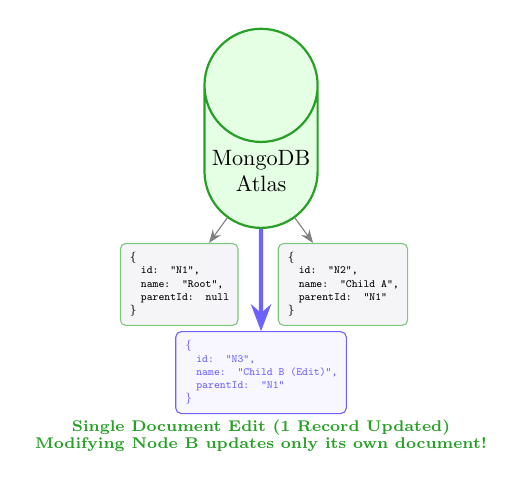
\begin{tikzpicture}[
          scale=0.8, every node/.style={transform shape},
          db/.style={cylinder, shape border rotate=90, draw=codegreen, fill=green!10, thick, minimum width=1.6cm, minimum height=1.0cm, align=center},
          jsonbox/.style={rectangle, draw=codegreen!60, fill=codebg, rounded corners=2pt, font=\ttfamily\tiny, align=left, inner sep=4pt}
        ]
          % DB cylinder
          \node[db] (database) at (0, 1.4) {MongoDB\\Atlas};
          
          % Flat node array
          \node[jsonbox] (n1) at (-1.3, -0.4) {
            \{ \\
            ~~id: "N1", \\
            ~~name: "Root", \\
            ~~parentId: null \\
            \}
          };
          \node[jsonbox] (n2) at (1.3, -0.4) {
            \{ \\
            ~~id: "N2", \\
            ~~name: "Child A", \\
            ~~parentId: "N1" \\
            \}
          };
          \node[jsonbox, draw=axonpurple, fill=axonpurple!5] (n3) at (0, -1.8) {
            \textcolor{axonpurple}{\textbf{\{}} \\
            ~~\textcolor{axonpurple}{\textbf{id: "N3",}} \\
            ~~\textcolor{axonpurple}{\textbf{name: "Child B (Edit)",}} \\
            ~~\textcolor{axonpurple}{\textbf{parentId: "N1"}} \\
            \textcolor{axonpurple}{\textbf{\}}}
          };
          
          \draw[-Stealth, gray] (database) -- (n1);
          \draw[-Stealth, gray] (database) -- (n2);
          \draw[-Stealth, axonpurple, line width=1.5pt] (database) -- (n3);
          
          \node[codegreen, align=center, font=\scriptsize\bfseries] at (0, -2.8) {
            \checkmark \textbf{Single Document Edit (1 Record Updated)} \\
            Modifying Node B updates only its own document!
          };
        \end{tikzpicture}
      \end{block}
    \end{column}
    \begin{column}{0.48\textwidth}
      \begin{block}{Client-Side Geometry Calculations}
        \centering
        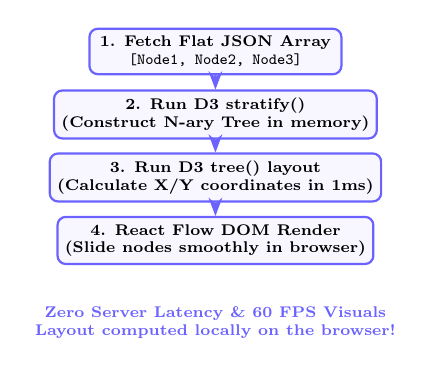
\begin{tikzpicture}[
          scale=0.8, every node/.style={transform shape},
          stepbox/.style={rectangle, draw=axonpurple, fill=axonpurple!5, thick, rounded corners=3pt, align=center, font=\scriptsize\bfseries, minimum width=4cm, minimum height=0.6cm},
          arrow/.style={-Stealth, thick, draw=axonpurple}
        ]
          % Flow steps
          \node[stepbox] (s1) at (0, 1.5) {1. Fetch Flat JSON Array \\ \texttt{[Node1, Node2, Node3]}};
          \node[stepbox] (s2) at (0, 0.5) {2. Run D3 stratify() \\ (Construct N-ary Tree in memory)};
          \node[stepbox] (s3) at (0, -0.5) {3. Run D3 tree() layout \\ (Calculate X/Y coordinates in 1ms)};
          \node[stepbox] (s4) at (0, -1.5) {4. React Flow DOM Render \\ (Slide nodes smoothly in browser)};
          
          \draw[arrow] (s1) -- (s2);
          \draw[arrow] (s2) -- (s3);
          \draw[arrow] (s3) -- (s4);
          
          \node[axonpurple, align=center, font=\scriptsize\bfseries] at (0, -2.8) {
            \checkmark \textbf{Zero Server Latency \& 60 FPS Visuals} \\
            Layout computed locally on the browser!
          };
        \end{tikzpicture}
      \end{block}
    \end{column}
  \end{columns}
\end{frame}

% ─── Slide 8: Advantage: Rich Node Context & Media ─────────────────────────
\begin{frame}{Rich Context: Media \& Attachment Support}
  Axon Flow treats mind map nodes as rich portals of information, going far beyond plain text label nodes:
  \vspace{0.5em}
  \begin{itemize}
    \item[\textcolor{axonpurple}{\tiny$\blacksquare$}] \textbf{File \& Code Attachments}:
      \begin{itemize}
        \item Users can upload PDFs, documents, or developer-centric source code files directly to any node.
        \item Stored securely via UUID-prefixed file upload API, with links embedded in the node document.
      \end{itemize}
    \item[\textcolor{axonpurple}{\tiny$\blacksquare$}] \textbf{Hyperlink Integrations}:
      \begin{itemize}
        \item Add multiple external hyperlinks per node, enabling references to tutorials, repositories, or documentations.
      \end{itemize}
    \item[\textcolor{axonpurple}{\tiny$\blacksquare$}] \textbf{Granular Inline Data}:
      \begin{itemize}
        \item Markdown-enabled note lists (\texttt{notes[]}) and status badges (e.g., \textit{reading}, \textit{revise}, \textit{completed}, \textit{important}) with custom visual indicators.
      \end{itemize}
  \end{itemize}
\end{frame}

% ─── Slide 9: Advantage: "Document-Wise" Reading View ───────────────────────
\begin{frame}{Outline Mode: Document-Wise Reading}
  One major problem with visual maps is \textbf{"canvas fatigue"} when trees get too deep. Axon Flow solves this with the \textbf{Document-Wise Reading View}:
  \vspace{0.8em}
  \begin{columns}
    \begin{column}{0.5\textwidth}
      \textbf{Linearized Concept Reading}:
      \begin{itemize}
        \item[\textcolor{axonpurple}{\tiny$\blacksquare$}] Toggles the map into a structured, sequential text document.
        \item[\textcolor{axonpurple}{\tiny$\blacksquare$}] Reconstructs the D3 tree into hierarchical headings (e.g., H1, H2, H3) based on depth.
        \item[\textcolor{axonpurple}{\tiny$\blacksquare$}] Renders notes, links, and code snippets inline, reading like a textbook or tutorial.
      \end{itemize}
    \end{column}
    \begin{column}{0.5\textwidth}
      \begin{block}{Why is it better for studying/reading?}
        \begin{enumerate}
          \item No panning or searching across the screen.
          \item Easier to read long notes and attachments.
          \item Combines the power of visual brainstorming with the clarity of linear documentation.
        \end{enumerate}
      \end{block}
    \end{column}
  \end{columns}
\end{frame}

% ─── Slide 10: Document-Wise Reading View Visualized ───────────────────────
\begin{frame}{Document-Wise Outline vs. Visual Canvas}
  \begin{columns}
    \begin{column}{0.48\textwidth}
      \begin{block}{Canvas Fatigue (Non-Linear View)}
        \centering
        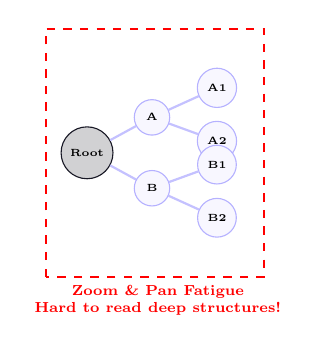
\begin{tikzpicture}[
          scale=0.75, every node/.style={transform shape},
          node/.style={circle, draw=axonpurple!50, fill=axonpurple!5, minimum size=0.6cm, font=\tiny\bfseries},
          root/.style={circle, draw=axondark, fill=axondark!20, minimum size=0.8cm, font=\tiny\bfseries}
        ]
          % Cluttered fanning tree (turned 90 degrees right)
          \node[root] (r) at (-1.5, 0.0) {Root};
          \node[node] (n1) at (-0.4, 0.6) {A};
          \node[node] (n2) at (-0.4, -0.6) {B};
          \node[node] (n3) at (0.7, 1.1) {A1};
          \node[node] (n4) at (0.7, 0.2) {A2};
          \node[node] (n5) at (0.7, -0.2) {B1};
          \node[node] (n6) at (0.7, -1.1) {B2};
          
          \draw[thick, axonpurple!40] (r) -- (n1);
          \draw[thick, axonpurple!40] (r) -- (n2);
          \draw[thick, axonpurple!40] (n1) -- (n3);
          \draw[thick, axonpurple!40] (n1) -- (n4);
          \draw[thick, axonpurple!40] (n2) -- (n5);
          \draw[thick, axonpurple!40] (n2) -- (n6);
          
          % Zoom/Pan indicator
          \draw[dashed, red, thick] (-2.2, -2.1) rectangle (1.5, 2.1);
          \node[red, align=center, font=\scriptsize\bfseries] at (-0.3, -2.5) {
            Zoom \& Pan Fatigue \\
            Hard to read deep structures!
          };
        \end{tikzpicture}
      \end{block}
    \end{column}
    \begin{column}{0.48\textwidth}
      \begin{block}{Linearized Outline (Document View)}
        \centering
        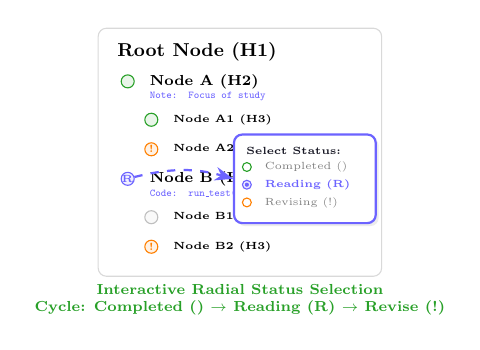
\begin{tikzpicture}[
          scale=0.75, every node/.style={transform shape},
          docbg/.style={rectangle, draw=gray!30, fill=white, rounded corners=3pt, minimum width=4.8cm, minimum height=4.2cm},
          heading1/.style={font=\bfseries\small, anchor=west},
          heading2/.style={font=\bfseries\scriptsize, anchor=west},
          heading3/.style={font=\bfseries\tiny, anchor=west},
          bodytext/.style={font=\ttfamily\tiny, color=gray, anchor=west}
        ]
          % Document background
          \node[docbg] (doc) at (0,0) {};
          
          % Document elements
          \node[heading1] at (-2.2, 1.7) {\textbf{Root Node (H1)}};
          
          % Node A (H2)
          \node[circle, draw=codegreen, fill=codegreen!10, minimum size=0.22cm, inner sep=0pt] (c1) at (-1.9, 1.2) {};
          \node[heading2] at (-1.65, 1.2) {Node A (H2)};
          \node[bodytext] at (-1.65, 0.95) {\textcolor{axonpurple}{Note: Focus of study}};
          
          % Node A1 (H3) - indented further
          \node[circle, draw=codegreen, fill=codegreen!10, minimum size=0.22cm, inner sep=0pt] (c11) at (-1.5, 0.55) {};
          \node[heading3] at (-1.25, 0.55) {Node A1 (H3)};
          
          % Node A2 (H3) - indented further
          \node[circle, draw=orange, fill=orange!10, minimum size=0.22cm, inner sep=0pt] (c12) at (-1.5, 0.05) {};
          \node[heading3] at (-1.25, 0.05) {Node A2 (H3)};
          
          % Node B (H2)
          \node[circle, draw=axonpurple, fill=axonpurple!10, minimum size=0.22cm, inner sep=0pt] (c2) at (-1.9, -0.45) {};
          \node[heading2] at (-1.65, -0.45) {Node B (H2)};
          \node[bodytext] at (-1.65, -0.7) {\textcolor{axonpurple}{Code: run\_test()}};
          
          % Node B1 (H3) - indented further
          \node[circle, draw=gray!50, fill=gray!5, minimum size=0.22cm, inner sep=0pt] (c21) at (-1.5, -1.1) {};
          \node[heading3] at (-1.25, -1.1) {Node B1 (H3)};
          
          % Node B2 (H3) - indented further
          \node[circle, draw=orange, fill=orange!10, minimum size=0.22cm, inner sep=0pt] (c22) at (-1.5, -1.6) {};
          \node[heading3] at (-1.25, -1.6) {Node B2 (H3)};
          
          % Labels inside status circles
          \node[font=\tiny\bfseries, codegreen] at (c1) {$\checkmark$};
          \node[font=\tiny\bfseries, codegreen] at (c11) {$\checkmark$};
          \node[font=\tiny\bfseries, orange] at (c12) {!};
          \node[font=\tiny\bfseries, axonpurple] at (c2) {R};
          \node[font=\tiny\bfseries, orange] at (c22) {!};
          
          % Manual Shadow for popover
          \node[fill=gray!15, rounded corners=3pt, minimum width=2.4cm, minimum height=1.5cm] at (1.15, -0.5) {};
          
          % Popover menu for status selection
          \node[draw=axonpurple, fill=white, rounded corners=3pt, thick, minimum width=2.4cm, minimum height=1.5cm] (popover) at (1.1, -0.45) {};
          
          % Popover elements
          \node[anchor=north west, font=\tiny\bfseries, color=axondark] (poptitle) at (popover.north west) [xshift=0.1cm, yshift=-0.1cm] {Select Status:};
          
          % Completed Option
          \node[circle, draw=codegreen, fill=white, minimum size=0.15cm, inner sep=0pt, anchor=west] (p1) at (popover.west) [xshift=0.15cm, yshift=0.2cm] {};
          \node[anchor=west, font=\tiny, color=gray] at (p1.east) [xshift=0.1cm] {Completed ($\checkmark$)};
          
          % Reading Option (selected)
          \node[circle, draw=axonpurple, fill=axonpurple!15, minimum size=0.15cm, inner sep=0pt, anchor=west] (p2) at (popover.west) [xshift=0.15cm, yshift=-0.1cm] {};
          \node[circle, fill=axonpurple, minimum size=0.07cm, inner sep=0pt] at (p2) {};
          \node[anchor=west, font=\tiny\bfseries, color=axonpurple] at (p2.east) [xshift=0.1cm] {Reading (R)};
          
          % Revising Option
          \node[circle, draw=orange, fill=white, minimum size=0.15cm, inner sep=0pt, anchor=west] (p3) at (popover.west) [xshift=0.15cm, yshift=-0.4cm] {};
          \node[anchor=west, font=\tiny, color=gray] at (p3.east) [xshift=0.1cm] {Revising (!)};
          
          % Arrow showing selection trigger from c2 to popover
          \draw[-Stealth, axonpurple, thick, dashed] (c2) to [bend left=15] (popover.west);
          
          \node[codegreen, align=center, font=\scriptsize\bfseries] at (0, -2.5) {
            \textbf{Interactive Radial Status Selection} \\
            Cycle: \textbf{Completed ($\checkmark$) $\rightarrow$ Reading (R) $\rightarrow$ Revise (!)}
          };
        \end{tikzpicture}
      \end{block}
    \end{column}
  \end{columns}
\end{frame}

% ─── Slide 11: Advantage: Bulleted-Text Bulk Import ─────────────────────────
\begin{frame}[fragile]{Bulleted-Text Outline Parser}
  Allows users to convert standard outline text files or lecture notes into interactive visual maps instantly.
  \vspace{0.5em}
  \begin{columns}
    \begin{column}{0.4\textwidth}
      \textbf{Indented Outlines Input:}
      \begin{lstlisting}[language=json, caption=Bulleted Text Outline]
Machine Learning
  Supervised
    Regression
    Classification
  Unsupervised
      \end{lstlisting}
    \end{column}
    \begin{column}{0.6\textwidth}
      \textbf{Stack-Based Indentation Parser:}
      \begin{itemize}
        \item[\textcolor{axonpurple}{\tiny$\blacksquare$}] Runs a line-by-line parser tracking indentation depth using a Stack structure.
        \item[\textcolor{axonpurple}{\tiny$\blacksquare$}] Automatically computes correct parent-child references.
        \item[\textcolor{axonpurple}{\tiny$\blacksquare$}] Generates all nodes and pushes them to the DB in a \textbf{single bulk API request} (\texttt{POST /api/nodes/bulk-create}).
      \end{itemize}
    \end{column}
  \end{columns}
\end{frame}

% ─── Slide 12: What is Optimistic UI? ───────────────────────────────────────
\begin{frame}{Optimistic UI: Mechanics \& Perceived Latency}
  \begin{center}
    \textit{"Don't make the user wait for the server. Assume success, render instantly."}
  \end{center}
  \vspace{0.5em}
  \begin{columns}
    \begin{column}{0.5\textwidth}
      \begin{block}{The Traditional Web Flow}
        \begin{enumerate}
          \item User clicks button.
          \item Spinner appears. Screen is frozen.
          \item Wait for network request (200ms -- 1.5s).
          \item Server confirms update in database.
          \item UI updates. Spinner disappears.
        \end{enumerate}
        \textit{Result}: Feels slow, clunky, and native-unfriendly.
      \end{block}
    \end{column}
    \begin{column}{0.5\textwidth}
      \begin{block}{The Optimistic UI Flow}
        \begin{enumerate}
          \item User clicks button.
          \item \textbf{UI updates instantly} based on expected success state.
          \item Network request is sent silently in background.
          \item If server succeeds: No change, keep editing.
          \item If server fails: \textbf{Rollback} UI to previous state and notify user.
        \end{enumerate}
        \textit{Result}: Feels instantaneous (0ms perceived latency).
      \end{block}
    \end{column}
  \end{columns}
\end{frame}

% ─── Slide 13: Optimistic UI vs. Traditional Flow Visualized ────────────────
\begin{frame}{Traditional Request vs. Optimistic UI Timelines}
  \begin{columns}
    \begin{column}{0.48\textwidth}
      \begin{block}{Traditional Flow Timeline}
        \centering
        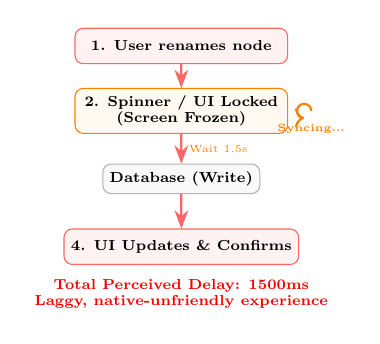
\begin{tikzpicture}[
          scale=0.75, every node/.style={transform shape},
          box/.style={rectangle, draw=red!60, fill=red!5, rounded corners=3pt, minimum width=3.6cm, minimum height=0.6cm, align=center, font=\scriptsize\bfseries},
          db/.style={rectangle, draw=gray!60, fill=gray!5, rounded corners=3pt, minimum width=2.4cm, minimum height=0.5cm, align=center, font=\scriptsize\bfseries},
          arrow/.style={-Stealth, thick, draw=red!60}
        ]
          % Timesteps
          \node[box] (t1) at (0, 2.0) {1. User renames node};
          \node[box, draw=orange, fill=orange!5] (t2) at (0, 0.9) {2. Spinner / UI Locked \\ (Screen Frozen)};
          \node[db] (t3) at (0, -0.25) {Database (Write)};
          \node[box] (t4) at (0, -1.4) {4. UI Updates \& Confirms};
          
          % Connections
          \draw[arrow] (t1) -- (t2);
          \draw[arrow] (t2) -- node[right, font=\tiny, color=orange]{Wait 1.5s} (t3);
          \draw[arrow] (t3) -- (t4);
          
          % Spinner drawing on the right of t2
          \draw[thick, orange, ->] (2.2, 0.9) arc (0:270:0.12);
          \node[orange, font=\tiny\bfseries] at (2.2, 0.6) {Syncing...};
          
          \node[red, align=center, font=\scriptsize\bfseries] at (0, -2.2) {
            Total Perceived Delay: \textbf{1500ms} \\
            Laggy, native-unfriendly experience
          };
        \end{tikzpicture}
      \end{block}
    \end{column}
    \begin{column}{0.48\textwidth}
      \begin{block}{Optimistic Flow Timeline}
        \centering
        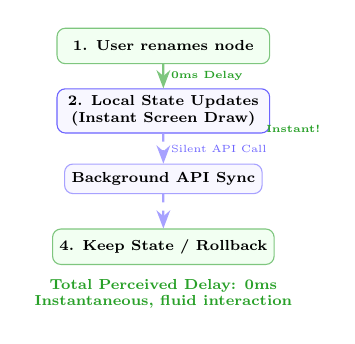
\begin{tikzpicture}[
          scale=0.75, every node/.style={transform shape},
          box/.style={rectangle, draw=codegreen!60, fill=green!5, rounded corners=3pt, minimum width=3.6cm, minimum height=0.6cm, align=center, font=\scriptsize\bfseries},
          db/.style={rectangle, draw=axonpurple!60, fill=axonpurple!5, rounded corners=3pt, minimum width=2.4cm, minimum height=0.5cm, align=center, font=\scriptsize\bfseries},
          arrow/.style={-Stealth, thick, draw=codegreen!60},
          bgarrow/.style={-Stealth, thick, dashed, draw=axonpurple!60}
        ]
          % Timesteps
          \node[box] (o1) at (0, 2.0) {1. User renames node};
          \node[box, draw=axonpurple, fill=axonpurple!5] (o2) at (0, 0.9) {2. Local State Updates \\ (Instant Screen Draw)};
          \node[db] (o3) at (0, -0.25) {Background API Sync};
          \node[box] (o4) at (0, -1.4) {4. Keep State / Rollback};
          
          % Connections
          \draw[arrow] (o1) -- node[right, font=\tiny, color=codegreen]{\textbf{0ms Delay}} (o2);
          \draw[bgarrow] (o2) -- node[right, font=\tiny, color=axonpurple]{Silent API Call} (o3);
          \draw[bgarrow] (o3) -- (o4);
          
          % Checkmark on the right of o2
          \node[codegreen, font=\bfseries\small] at (2.2, 0.9) {$\checkmark$};
          \node[codegreen, font=\tiny\bfseries] at (2.2, 0.6) {Instant!};
          
          \node[codegreen, align=center, font=\scriptsize\bfseries] at (0, -2.2) {
            Total Perceived Delay: \textbf{0ms} \\
            Instantaneous, fluid interaction
          };
        \end{tikzpicture}
      \end{block}
    \end{column}
  \end{columns}
\end{frame}

% ─── Slide 14: Optimistic UI: Renaming a Node ───────────────────────────────
\begin{frame}[fragile]{Optimistic UI: Node Rename Implementation}
  When a user renames a node bubble on the canvas and presses \texttt{Enter}:
  \vspace{0.2em}
  \begin{columns}
    \begin{column}{0.55\textwidth}
      \textbf{Local State Update Logic}:
      \begin{lstlisting}[language=javascript]
// 1. Immediately modify local flat state
setBackendNodes(prevNodes => 
  prevNodes.map(node => {
    if (node.id === targetId) {
      return { ...node, name: newName }; // New obj
    }
    return node; // Unchanged references kept
  })
);

// 2. Fire the API call silently in the background
nodeApi.renameNode(targetId, newName)
  .catch(err => {
    // 3. Rollback logic if backend fails
    revertLocalState(previousNodes);
  });
      \end{lstlisting}
    \end{column}
    \begin{column}{0.45\textwidth}
      \textbf{Background Pipeline}:
      \begin{enumerate}
        \item User finishes editing inline.
        \item State changes immediately.
        \item Re-runs React-D3 rendering cycle, adjusting node coordinates.
        \item Server updates the MongoDB document in the background.
        \item The user experiences zero interruption or delay.
      \end{enumerate}
    \end{column}
  \end{columns}
\end{frame}

% ─── Slide 15: Optimistic UI: Adding a Child Node ──────────────────────────
\begin{frame}[fragile]{Optimistic UI: Temporary Child Draft Nodes}
  Adding a new child is complex because we do not have a MongoDB \texttt{\_id} key until the server responds, yet the canvas must render the new node instantly.
  \vspace{0.4em}
  \begin{columns}
    \begin{column}{0.5\textwidth}
      \textbf{Phase 1: Temporary Draft Node}
      \begin{itemize}
        \item Creates a client-only node with a temporary ID: \texttt{`draft-\$\{Date.now()\}`}.
        \item Injected into the flat list state instantly.
        \item D3 engine runs, pushes existing nodes away to make room, and displays an input textbox.
      \end{itemize}
    \end{column}
    \begin{column}{0.5\textwidth}
      \textbf{Phase 2: Confirmed Swap-Out}
      \begin{itemize}
        \item User hits Enter $\rightarrow$ \texttt{POST} request sent.
        \item Server creates MongoDB record and returns real ObjectId.
        \item Frontend swaps the draft node object with the real node in state using \texttt{map()}.
        \item Transition is completely invisible to the user.
      \end{itemize}
    \end{column}
  \end{columns}
\end{frame}

% ─── Slide 16: Optimistic UI: Drag-and-Drop Reparenting ────────────────────
\begin{frame}{Optimistic UI: Drag-and-Drop Reparenting}
  Dragging one node and dropping it onto another changes its parent relationship.
  \vspace{0.4em}
  \begin{columns}
    \begin{column}{0.55\textwidth}
      \textbf{The Interaction Algorithm}:
      \begin{enumerate}
        \item \textbf{Hit-Test (Dragging)}: A bounding box check (+24px offset) determines if the dragged node is hovering over another node.
        \item \textbf{Cycle Prevention}: Prevents drops on its own child nodes or itself.
        \item \textbf{Target Highlight}: Blue pulsing ring indicator.
        \item \textbf{Optimistic State Update}: On drop release, the node's \texttt{parentId} is instantly changed in the local state, triggering a redraw.
        \item \textbf{Persist \& Rollback}: Backend is updated in background. If it fails, the frontend issues a full re-fetch to restore the old state.
      \end{enumerate}
    \end{column}
    \begin{column}{0.45\textwidth}
      \begin{center}
        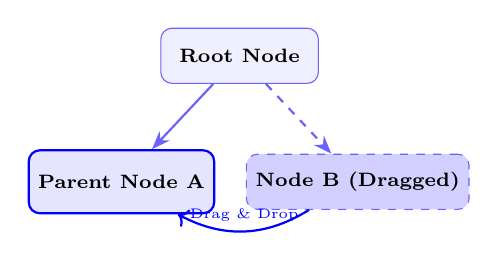
\begin{tikzpicture}[
          node/.style={rectangle, draw=axonpurple, fill=axonpurple!10, rounded corners, minimum width=2cm, minimum height=0.7cm, font=\scriptsize\bfseries},
          activeNode/.style={rectangle, draw=axonpurple, fill=axonpurple!30, rounded corners, minimum width=2cm, minimum height=0.7cm, font=\scriptsize\bfseries, dashed},
          targetNode/.style={rectangle, draw=blue, fill=blue!10, thick, rounded corners, minimum width=2.2cm, minimum height=0.8cm, font=\scriptsize\bfseries},
          flow/.style={-Stealth, thick, draw=axonpurple}
        ]
          \node[node] (root) at (0, 1.8) {Root Node};
          \node[targetNode] (nodeA) at (-1.5, 0.2) {Parent Node A};
          \node[activeNode] (nodeB) at (1.5, 0.2) {Node B (Dragged)};
          
          \draw[flow] (root) -- (nodeA);
          \draw[flow, dashed] (root) -- (nodeB);
          \draw[flow, ->, blue, bend left] (nodeB) to node[above, font=\tiny]{Drag \& Drop} (nodeA);
        \end{tikzpicture}
      \end{center}
    \end{column}
  \end{columns}
\end{frame}

% ─── Slide 17: Why the Screen Doesn't Flash (React Diffing) ─────────────────
\begin{frame}[fragile]{DOM Reconciliation: Preventing Screen Flicker}
  Every time layout math recalculates coordinates for all nodes in the tree, you would expect the browser to reload or flicker. It does not. Here is why:
  \vspace{0.4em}
  \begin{columns}
    \begin{column}{0.5\textwidth}
      \begin{block}{1. Math vs. Visuals}
        D3-Hierarchy layout updates coordinates strictly in memory (taking less than \textbf{1 millisecond}). It does not touch the HTML elements directly.
      \end{block}
    \end{column}
    \begin{column}{0.5\textwidth}
      \begin{block}{2. React Flow Virtual DOM Diffing}
        React Flow compares node IDs in the old and new arrays. It updates only the CSS inline styles, sliding elements smoothly.
      \end{block}
    \end{column}
  \end{columns}
  \vspace{0.2em}
  \textbf{React Flow DOM Translation Output}:
  \begin{lstlisting}[language=html]
  <!-- BEFORE: X=100, Y=150 -->
  <div class="react-flow__node" data-id="NODE_2" style="transform: translate(100px, 150px);">
  
  <!-- AFTER DIFFING: X=50, Y=150 (Only the translate coordinate is modified in DOM) -->
  <div class="react-flow__node" data-id="NODE_2" style="transform: translate(50px, 150px);">
  \end{lstlisting}
\end{frame}

% ─── Slide 18: Reactivity Loop: Math \& Diffing Visualized ────────────────
\begin{frame}[fragile]{Coordinate Math \& Virtual DOM Diffing}
  \begin{columns}
    \begin{column}{0.45\textwidth}
      \begin{block}{1. D3 Coordinate Calculation}
        \textbf{Flat JSON Input (parentId refs):}
        \begin{lstlisting}[language=json, basicstyle=\ttfamily\tiny]
[
  {"id": "N1", "parentId": null},
  {"id": "N2", "parentId": "N1"}
]
        \end{lstlisting}
        \vspace{0.3em}
        \textbf{D3 Stratify \& Tree Calculation:}
        \begin{itemize}
          \item[\textcolor{axonpurple}{\tiny$\blacksquare$}] Runs \texttt{d3.stratify()} in memory.
          \item[\textcolor{axonpurple}{\tiny$\blacksquare$}] Calculates layout node positions in <1ms.
        \end{itemize}
        \vspace{0.3em}
        \textbf{Layout JSON Output (X/Y coordinates):}
        \begin{lstlisting}[language=json, basicstyle=\ttfamily\tiny]
[
  {"id": "N1", "x": 0, "y": 0},
  {"id": "N2", "x": 100, "y": 50}
]
        \end{lstlisting}
      \end{block}
    \end{column}
    
    \begin{column}{0.53\textwidth}
      \begin{block}{2. React Flow DOM Diffing}
        \centering
        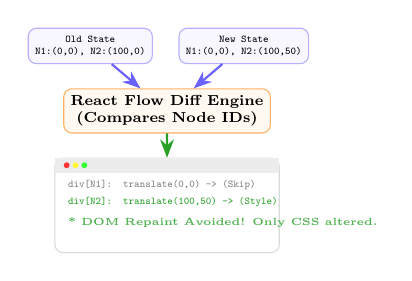
\begin{tikzpicture}[
          scale=0.75, every node/.style={transform shape},
          statebox/.style={rectangle, draw=axonpurple!50, fill=axonpurple!5, rounded corners=3pt, minimum width=2.0cm, minimum height=0.6cm, align=center, font=\tiny\ttfamily},
          diffbox/.style={rectangle, draw=orange!60, fill=orange!5, rounded corners=3pt, minimum width=3.0cm, minimum height=0.6cm, align=center, font=\scriptsize\bfseries},
          browserbox/.style={rectangle, draw=gray!30, fill=white, rounded corners=3pt, minimum width=3.8cm, minimum height=1.6cm}
        ]
          % States
          \node[statebox] (oldstate) at (-1.3, 1.9) {Old State\\N1:(0,0), N2:(100,0)};
          \node[statebox] (newstate) at (1.3, 1.9) {New State\\N1:(0,0), N2:(100,50)};
          
          % Diff Engine
          \node[diffbox] (diff) at (0, 0.8) {React Flow Diff Engine\\(Compares Node IDs)};
          
          % Browser DOM Mockup
          \node[browserbox] (browser) at (0, -0.8) {};
          \fill[gray!15] (-1.9, 0.0) rectangle (1.9, -0.25);
          \fill[red!80] (-1.7, -0.12) circle (0.05);
          \fill[yellow!80] (-1.55, -0.12) circle (0.05);
          \fill[green!80] (-1.4, -0.12) circle (0.05);
          
          \node[anchor=west, font=\tiny\ttfamily, color=gray] at (-1.8, -0.45) {div[N1]: translate(0,0) -> (Skip)};
          \node[anchor=west, font=\tiny\ttfamily, color=codegreen] at (-1.8, -0.75) {div[N2]: translate(100,50) -> (Style)};
          \node[anchor=west, font=\tiny\bfseries, color=codegreen!80] at (-1.8, -1.1) {* DOM Repaint Avoided! Only CSS altered.};
          
          % Connections
          \draw[-Stealth, thick, axonpurple] (oldstate) -- (diff);
          \draw[-Stealth, thick, axonpurple] (newstate) -- (diff);
          \draw[-Stealth, thick, codegreen] (diff) -- (browser);
        \end{tikzpicture}
      \end{block}
    \end{column}
  \end{columns}
\end{frame}

% ─── Slide 19: Render Performance: Complexity \& Scalability Limits ────────
\begin{frame}{Render Performance: Complexity \& Scalability Limits}
  \begin{columns}
    \begin{column}{0.5\textwidth}
      \begin{block}{Time Complexity Analysis}
        \begin{itemize}
          \item[\textcolor{axonpurple}{\tiny$\blacksquare$}] \textbf{D3 Layout Math}: $\mathbf{O(N)}$
            \begin{itemize}
              \item Tree reconstruction \& layout traversal.
              \item In-memory math takes \textbf{< 1ms} for 500 nodes.
            \end{itemize}
          \vspace{0.2em}
          \item[\textcolor{axonpurple}{\tiny$\blacksquare$}] \textbf{Virtual DOM Diffing}: $\mathbf{O(N)}$
            \begin{itemize}
              \item React compares node IDs using key references.
            \end{itemize}
          \vspace{0.2em}
          \item[\textcolor{axonpurple}{\tiny$\blacksquare$}] \textbf{Browser Reflow \& Paint}: $\mathbf{O(N \log N)}$
            \begin{itemize}
              \item Linear reflow (absolute positioning), but SVG edge updates increase paint overhead.
            \end{itemize}
        \end{itemize}
      \end{block}
    \end{column}
    
    \begin{column}{0.5\textwidth}
      \begin{block}{Why it degrades (>500 nodes)}
        \begin{itemize}
          \item \textbf{DOM Node Overload}: 500+ HTML divs + SVG paths exceed browser GPU paint budget.
          \item \textbf{Frame Budget Breached}: Drag updates trigger reflows, exceeding the \textbf{16.6ms budget} (FPS drops).
        \end{itemize}
      \end{block}
      \vspace{-0.2em}
      \begin{block}{Advanced Optimizations}
        \begin{itemize}
          \item \textbf{Viewport Virtualization}: Render only nodes visible in the viewport.
          \item \textbf{Canvas/WebGL Rendering}: Bypass DOM by painting directly to Canvas buffer (5,000+ nodes).
          \item \textbf{Web Workers}: Run layout math off the main thread.
        \end{itemize}
      \end{block}
    \end{column}
  \end{columns}
\end{frame}

% ─── Slide 20: Generative AI: Local Node & Map Expansion ──────────────────
\begin{frame}{Local Generative AI: Node Expansion \& Auto-Mapping}
  Axon Flow integrates a local AI assistant to automate brainstorming and map creation, without relying on cloud APIs.
  \vspace{0.4em}
  \begin{columns}
    \begin{column}{0.5\textwidth}
      \begin{block}{AI Core Capabilities (Planned)}
        \begin{itemize}
          \item[\textcolor{axonpurple}{\tiny$\blacksquare$}] \textbf{Contextual Node Expansion}: Select any node and trigger the AI to generate 4--6 relevant subtopics as children.
          \item[\textcolor{axonpurple}{\tiny$\blacksquare$}] \textbf{Prompt-to-Map (Auto-Map)}: Input a single topic prompt (e.g., \textit{"Deep Learning Basics"}) to spawn a multi-level tree.
        \end{itemize}
      \end{block}
    \end{column}
    \begin{column}{0.5\textwidth}
      \begin{block}{User-Controlled Permissions}
        Allows enabling/disabling AI tool access:
        \begin{itemize}
          \item \textbf{Web Search}: LLM searches DuckDuckGo for live facts.
          \item \textbf{File Reader}: LLM searches DuckDuckGo/local files for attached data.
        \end{itemize}
      \end{block}
    \end{column}
  \end{columns}
\end{frame}

% ─── Slide 21: Local AI Capabilities Visualized ─────────────────────────────
\begin{frame}{AI Expansion \& Tool Permission Controls}
  \begin{columns}
    \begin{column}{0.48\textwidth}
      \begin{block}{AI Map Expansion (Contextual \& Auto-Map)}
        \centering
        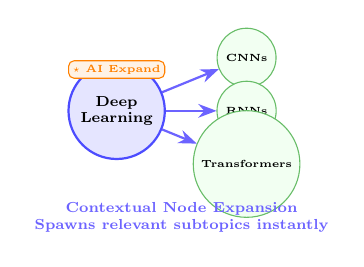
\begin{tikzpicture}[
          scale=0.75, every node/.style={transform shape},
          rootnode/.style={circle, draw=blue!70, fill=blue!10, thick, minimum size=1.0cm, align=center, font=\scriptsize\bfseries},
          childnode/.style={circle, draw=codegreen!70, fill=green!5, minimum size=0.8cm, align=center, font=\tiny\bfseries},
          arrow/.style={-Stealth, thick, draw=axonpurple}
        ]
          % Selected Parent Node
          \node[rootnode] (p) at (-1.3, 0.0) {Deep\\Learning};
          
          % AI expand trigger badge
          \node[draw=orange, fill=orange!10, rounded corners=2pt, font=\tiny\bfseries, text=orange, inner sep=2pt] at (-1.3, 0.7) {$\star$ AI Expand};
          
          % AI Generated Children
          \node[childnode] (c1) at (0.9, 0.9) {CNNs};
          \node[childnode] (c2) at (0.9, 0.0) {RNNs};
          \node[childnode] (c3) at (0.9, -0.9) {Transformers};
          
          % Connections
          \draw[arrow] (p) -- (c1);
          \draw[arrow] (p) -- (c2);
          \draw[arrow] (p) -- (c3);
          
          \node[axonpurple, align=center, font=\scriptsize\bfseries] at (-0.2, -1.8) {
            Contextual Node Expansion \\
            Spawns relevant subtopics instantly
          };
        \end{tikzpicture}
      \end{block}
    \end{column}
    
    \begin{column}{0.48\textwidth}
      \begin{block}{AI Tool Permissions Panel}
        \centering
        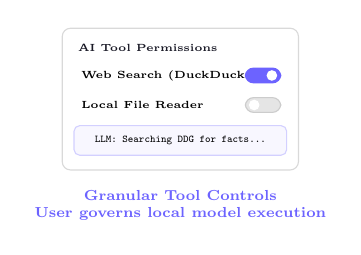
\begin{tikzpicture}[
          scale=0.75, every node/.style={transform shape},
          panelbox/.style={rectangle, draw=gray!30, fill=white, rounded corners=3pt, minimum width=4.0cm, minimum height=2.4cm},
          togglepill_on/.style={rectangle, draw=axonpurple, fill=axonpurple, rounded corners=3pt, minimum width=0.6cm, minimum height=0.25cm, inner sep=0pt},
          togglepill_off/.style={rectangle, draw=gray!40, fill=gray!20, rounded corners=3pt, minimum width=0.6cm, minimum height=0.25cm, inner sep=0pt},
          togglecircle/.style={circle, fill=white, minimum size=0.18cm, inner sep=0pt},
          statusbox/.style={rectangle, draw=axonpurple!30, fill=axonpurple!5, rounded corners=2pt, minimum width=3.6cm, minimum height=0.5cm, align=left, font=\tiny\ttfamily}
        ]
          % Panel background
          \node[panelbox] (panel) at (0, 0) {};
          \node[anchor=north west, font=\tiny\bfseries, color=axondark] at (panel.north west) [xshift=0.15cm, yshift=-0.15cm] {AI Tool Permissions};
          
          % Toggle 1: Web Search (ON)
          \node[anchor=west, font=\tiny\bfseries] at (-1.8, 0.4) {Web Search (DuckDuckGo)};
          \node[togglepill_on] (t1) at (1.4, 0.4) {};
          \node[togglecircle] at (1.55, 0.4) {};
          
          % Toggle 2: File Reader (OFF)
          \node[anchor=west, font=\tiny\bfseries] at (-1.8, -0.1) {Local File Reader};
          \node[togglepill_off] (t2) at (1.4, -0.1) {};
          \node[togglecircle] at (1.25, -0.1) {};
          
          % Active Tool Status Log
          \node[statusbox] (status) at (0, -0.7) {LLM: Searching DDG for facts...};
          
          \node[axonpurple, align=center, font=\scriptsize\bfseries] at (0, -1.8) {
            Granular Tool Controls \\
            User governs local model execution
          };
        \end{tikzpicture}
      \end{block}
    \end{column}
  \end{columns}
\end{frame}

% ─── Slide 22: AI Implementation & SSE Streaming Pipeline ──────────────────
\begin{frame}[fragile]{FastAPI SSE Streaming \& JSON Parser}
  To avoid freezing the UI during LLM inference, Axon Flow streams responses using a FastAPI-based AI engine:
  \vspace{0.3em}
  \begin{center}
    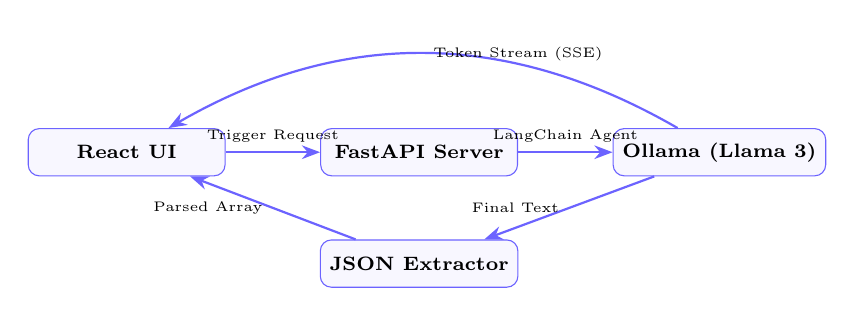
\begin{tikzpicture}[
      node distance=0.8cm and 1.2cm,
      box/.style={rectangle, rounded corners=4pt, draw=axonpurple, fill=axonpurple!5, minimum width=2.5cm, minimum height=0.6cm, align=center, font=\scriptsize\bfseries},
      arrow/.style={-Stealth, thick, draw=axonpurple}
    ]
      \node[box] (fe) at (0,0) {React UI};
      \node[box, right=of fe] (api) {FastAPI Server};
      \node[box, right=of api] (ollama) {Ollama (Llama 3)};
      \node[box, below=of api] (parser) {JSON Extractor};
      
      \draw[arrow] (fe) -- node[above, font=\tiny]{Trigger Request} (api);
      \draw[arrow] (api) -- node[above, font=\tiny]{LangChain Agent} (ollama);
      \draw[arrow, bend right] (ollama) to node[right, font=\tiny]{Token Stream (SSE)} (fe);
      \draw[arrow] (ollama) -- node[left, font=\tiny]{Final Text} (parser);
      \draw[arrow] (parser) -- node[left, font=\tiny]{Parsed Array} (fe);
    \end{tikzpicture}
  \end{center}
  \vspace{-0.5em}
  \begin{itemize}
    \item[\textcolor{axonpurple}{\tiny$\blacksquare$}] \textbf{SSE Streaming Protocol}: Emits raw text tokens to React's \texttt{EventSource} in real-time.
    \item[\textcolor{axonpurple}{\tiny$\blacksquare$}] \textbf{JSON Schema Extraction}: Regex-based fallback parser extracts structured array formats from the LLM outputs and maps them into hierarchical parent-child nodes.
  \end{itemize}
\end{frame}

% ─── Slide 23: Competitive Analysis: How Axon Flow Compares ───────
\begin{frame}{Competitive Analysis: Miro/XMind vs. Axon Flow}
  \centering
  \begin{tabularx}{\textwidth}{lXX}
    \toprule
    \textbf{Dimension} & \textbf{Traditional Tools (Miro / XMind)} & \textbf{Axon Flow} \\
    \midrule
    \textbf{Data Privacy} & High risk; data uploaded to cloud LLMs (OpenAI/Anthropic). & \textbf{100\% private}; runs local model offline via Ollama. \\
    \midrule
    \textbf{Tech Integrations} & Plain text only; no developer attachment capability. & Bind \textbf{source code, attachments}, and links to nodes. \\
    \midrule
    \textbf{Reading Experience} & Panning/zooming fatigue on deep visual maps. & Dual view: Switch to linear \textbf{Document-Wise Outlines}. \\
    \midrule
    \textbf{Render Performance} & Heavy HTML/canvas redraws causing drag lags. & Optimized flat MongoDB schema + React Virtual DOM translation. \\
    \bottomrule
  \end{tabularx}
\end{frame}

% ─── Slide 24: Summary: The Smart Client, Dumb Server Pattern ──────────────
\begin{frame}{Architectural Pattern: Smart Client, Dumb Server}
  Axon Flow uses the \textbf{"Smart Client, Dumb Server"} pattern to optimize network load and visual smoothness:
  \vspace{0.8em}
  \begin{table}
    \centering
    \begin{tabular}{p{0.45\textwidth} p{0.45\textwidth}}
      \toprule
      \textbf{The Dumb Backend (Express + MongoDB)} & \textbf{The Smart Frontend (React + D3)} \\
      \midrule
      \begin{itemize}
        \item Simply records relationships.
        \item Serves flat lists.
        \item Handles secure authentication and uploads.
      \end{itemize}
      &
      \begin{itemize}
        \item Computes layouts and positions dynamically.
        \item Renders fluid drag-and-drop visuals.
        \item Enables zero-delay Optimistic UI.
      \end{itemize}
      \\ \bottomrule
    \end{tabular}
  \end{table}
\end{frame}

% ─── Slide 25: Conclusion & Takeaways ──────────────────────────────────────
\begin{frame}{Conclusion \& Technical Summary}
  \begin{block}{Key Technical Accomplishments}
    \begin{itemize}
      \item[\checkmark] \textbf{Performance}: Up to 500 nodes rendered smoothly at 60 FPS by running D3 math on client-side and using React Virtual DOM diffs.
      \item[\checkmark] \textbf{Zero Perceived Latency}: Dynamic Optimistic UI updates for creation, renaming, and reparenting actions.
      \item[\checkmark] \textbf{Robust Data Model}: Flat independent node document design in MongoDB scales infinitely better than nested trees.
      \item[\checkmark] \textbf{Enhanced Context}: Attach links, code files, and view outlines in the Document-Wise reader.
    \end{itemize}
  \end{block}
  \vspace{0.5em}
  \begin{center}
    \textbf{Thank You! Questions?}
  \end{center}
\end{frame}

\end{document}
